\section{Evaluation of real-time interactions between the user and the agent}
\label{sec:eval}

%We present in this section an evaluation of an embodied conversational agent coordinating turns in real time with users in the context of a negociation scenario.

\subsection{Motivation}

This evaluation aimed at answering three questions: 
%\begin{enumerate}
%\item
(i) Is an agent controlled by our turn-taking model able to coordinate smoothly its speaking turns with the user?
%\item
(ii) Is an agent controlled by our turn-taking model able to correctly signal its intentions (either taking, yielding keeping or grabbing the turn) to the user?
%\item
(iii) Can an agent varying its turn-taking behavior according to our model improve judgements about the agent's credibility, user's satisfaction and easiness to interact with the agent?
%\end{enumerate}

%To that purpose we chose to inspire from 
Our methodology was based on existing evaluations techniques.
\cite{skantze_towards_2010} and \cite{de_vault_toward_2015} conducted two studies to evaluate agent's turn-taking in the context of negociation scenarios. In these two experiments, the agents were at least partially controlled by a Wizard of Oz (WOz). In \cite{skantze_towards_2010} only the user's utterances were transcribed by the WOz, the remaining being managed by the system. User's end of turns were identified using a voice activity detector and the system systematically responded to the user after detecting the end of the user's turn. In \cite{de_vault_toward_2015}, the whole process, from interpretation to generation, was managed by the Wizard of Oz, including turn-taking management. These two experiments had the advantage to answer similar research questions as ours regarding turn-taking. First, the ability of the agent to coordinate with the user was evaluated by comparisons of the agent's response time and overlap duration with human interactions. Second, the agent's credibility, the user's satisfaction and easiness to interact with the agent were evaluated through questionnaire. The ability of the agent to correctly signals its intentions towards turn-taking was not directly treated. However some behaviors of the user were analyzed in these evaluations such as the user latency to take the turn after the end of the agent's turn. To our view, these behavior could be related to the ability of the user to clearly identify signals displayed by the agent, the clearer the agent's signals, the shorter the user's response latencies. As these evaluations seemed particularly adapted to our own goals, we chose to inspire from them to elaborate our own evaluation. One major difference is that, in our case, the agent's turn-taking behaviors varied according to the output our model. 

\subsection{Protocol}

Similarly to \cite{de_vault_toward_2015} and \citep{skantze_towards_2010}, we conducted an experiment where the user was engaged in a negociation scenario with an agent. The interaction was only audio, the agent had no graphical representation and only perceived and controlled two prosodic parameters, the loudness and the pitch. 
%In the negociation scenario, both participants are on a sinking boat, and prepare to 
The scenario stages two participants on board a sinking boat, preparing to embark on a life boat. 
Each participant has different beliefs on the situation. 
One thinks that they are close to the coast, in this situation the priority is then to reach the coast as fast as possible. 
The other thinks they are far from the coast, the priority being here to survive as long as possible. 
Given their different beliefs, they have to make a share decision about three items to take away in the life boat among six. We chose the different items such as three of them were adapted to first situation 
%where participants are close to the coast 
and three to the second one.
objects were adapted to situations were participants are far from the coast. 
The scenario conducted the user, given his own belief, to disagree with the agents' proposals.   
% Déplacé en second paragraphe

We used our implementation presented in section \ref{impl}. The agent had thus a complete turn-taking module that determined when the agent utterance should be launched. In order to avoid user's utterances misinterpretations we chose to replace the Automatic Speech Recognizer and Response Planning components by a Wizard of Oz. The WOz listened and selected utterances thanks to an interface that allowed to select arguments in favor of the items the agent wanted to take and to produce counter-arguments to the user's proposals. It was necessary to avoid any influence of the Wizard of Oz response time on the agent turn-taking behavior. To that purpose, the WOz was instructed to select the agent's next utterance before the end of the user's utterance. 
To make the WOz answering as fast as possible, the interface was organised in buttons, determining the different dialog acts. Once the Wizard of Oz selected a particular dialog act by clicking the corresponding button, an utterance related to this dialog act was chosen among a list of utterances, allowing the agent to vary its answers to the user. The utterance chosen was then sent to the agent that determined when to launch the utterance according to the output of the turn-taking module, using the mechanism presented in section \ref{impl}. In order to have the most natural interactions, the different utterances that the agent could produced were collected from a corpus of human interactions we collected before. 

%À caser
%. 

% Déplacé en troisième paragraphe
%In order to assess the ability of our agent to coordinate with the user, 
We compared our turn-taking model (M1) with an implementation of a second model (M2). 
In this second model, we used a voice activity detector to discriminate moments when the user spoke from moment of silence. 
%Given the result of the voice activity detector,
The second turn-taking module was implemented following the following rules: 
\begin{itemize}
\item when no speech activity is detected after 600~ms, consider that the user has finished its turn and take the turn;
\item after at least 100~ms of speech activity, consider that the user is beginning a new turn and stop speaking. 
\end{itemize} 
These rules based on temporal threshold are often used in spoken dialog systems and agent architectures. 
Interestingly, they are considered as non-optimal \citep{ward_root_2005}. 
The two thresholds of 600~ms and 100~ms corresponded to values used in existing models (see for example \citep{ferrer_is_2002}). 

When the agent was controlled by our model M1, it was able to modulate its prosodic signals and thus to inform the user about its intentions by decreasing the pitch and loudness of its voice at the end of the turn and raising its pitch and loudness to inform the user about its intention to grab the turn.  
With model M2, the agent was not able to vary its prosodic signals and thus had no modality to convey any information about its intention. 

The values of the motivation parameter $m$ were set such as according to its current role, the agent had two possible turn-taking behavior. In the first case, the agent had a weak motivation to keep the turn as a speaker ($m=-0.4$) making it releasing the turn when it detected that the user wanted to grab the turn, and a weak motivation to take the turn as a listener making it waiting the end of the user's turn before taking the turn. In the second case, the agent had a strong motivation to keep the turn ($m=-1.0$), making it insisting to keep the turn when it detected that the user wanted to grab the turn, and a strong motivation to take the turn ($m=1.0$), making it to systematically trying to grab the turn. 

We ensured that the user interacted equally with the agent having respectively weak and strong motivation to take or keep the turn. To that purpose, we divided the interaction in two parts. In the first part the user interacted with an agent having a weak motivation to take or keep the turn, and in the second part with an agent with a strong motivation.
% the user interacted with an agent having a strong motivation to take and keep the turn. 
We kept this order for all the interactions, because beginning the interaction with an agent systematically trying to grab or to keep the turn would risk to make the user to refuse to continue to engage in the interaction with the agent. 

%As a result, we had two main conditions,
The different conditions of the experiment were as follows.
In condition 1 the user interacted with an agent controlled by model M1.
In condition 2, the user interacted with an agent controlked by model M2.
Condition 1 presented to variants, depending of the value of the motivation parameter: ``condition 1 strong'' and ``condition 1 weak''. 
% We chose to name the first part of the condition 1, when the user interacted with an agent having a weak motivation to keep and take the turn ``condition 1 weak", and the second part of the ``condition 1 strong", when the user interacted with an agent having a weak motivation to keep and take the turn ``condition 1 strong". 
Each participant interacted twice with the agent, each time with a different condition.
The order of the conditions (``condition 1" and ``condition 2") was counterbalanced between participants.
For each condition, the interaction lasted 2 min 30 s. 

At the end of each interaction, a questionnaire, presented table \ref{Answers}, was proposed to the participant, with questions about the easiness to interact with the agent (question Q9 in table \ref{Answers}), user's satisfaction (Q8, Q10) and agent credibility (Q11). The corresponding questions were adapted from \cite{skantze_towards_2010}, \cite{bevacqua_effects_2014} and \cite{de_vault_toward_2015}. Moreover, in order to assess the clarity of the agent's signals, we added questions about the intentionality of agent's interruptions that is whether interruptions of the agent were due to an agent mistakenly perceiving the end of turn of the user or where made by the agent on purpose (Q3, Q4). Finally, we added questions about the ability of the agent to smoothly coordinate with the user (Q1, Q2, Q6, Q7).
For each items, the participant had to declare its level of agreement, between strongly disagree and strongly agree in a continuous scale between 0 à 10 The different items were inspired from \cite{skantze_towards_2010}, \cite{bevacqua_effects_2014} and \cite{de_vault_toward_2015}.

\section{Results}

31 volonteers (30 men and 1 woman) participated to the experiment. They were all native French speakers and were students, engineers or researchers. The results to the questionnaire for condition 1 and condition 2 are shown on Table \ref{Answers}. 
\begin{table}
\centering
\resizebox{\linewidth}{!}{\begin{tabular}{|p{3cm}|p{2cm}|p{2cm}|p{2cm}|}
\hline
Questions & Median \linebreak conds. 1 & Median \linebreak cond. 2 & p-value \\
\hline
Q1: My interlocutor \linebreak didn't perceive the moment were I talked & 2.25 & 1.75 & 0.95\\
\hline
Q2: My interlocutor took the turn randomly& 2.5 & 2.625 & 0.6 \\
\hline
Q3: My interlocutor interrupted unvolontarily& 6 & 4 & 0.019* \\
\hline
Q4: My interlocutor interrupted me on purpose& 6 & 6.5 & 0.91 \\
\hline
Q5: My interlocutor paid attention not to interrupt me & 4.5 & 7.5 & 0.006**\\
\hline
Q6: My interlocutor was slow to respond to me & 3 & 2 & 0.77\\
\hline
Q7: My interlocutor refused sometimes to speak to me & 6.125 & 5.75 & 0.16\\
\hline
Q8: My interlocutor annoyed me by the way he took the turn & 4.5 & 3.25 & 0.54\\
\hline
Q9: I was at ease interacting with my interlocutor & 5.25 & 6.25 & 0.55\\
\hline
Q10: I liked speaking with my interlocutor & 6.625 & 7 & 0.52\\
\hline
Q11: The behavior of my interlocutor was close to the behavior of a human speaker & 5.625 & 6.5 & 0.97\\
\hline
\end{tabular}}
\caption{Mean agreements of the participants for conditions 1 and condition 2 (translated from French).}
\label{Answers}
\end{table}

%In this table are translated the different assertions of the question, the mean responses of the participants, and the significance of differences in the responses between the two conditions. 
Generally speaking, the participants liked speaking with the agent (question Q10). The results of the question related to the credibility of the agent are more mitigated (Q11), with a median value to the assertion "The behavior of my interlocutor was close to the behavior of a human speaker" of 6.5 in the second condition and 5.625 for the first condition. The users perceived that the agent paid more attention not to interrupt them (median value of 7.5 for Q5) for the second condition than for the first one. Nevertheless, participants perceived also counter-intuitively that the agent interrupted them more unvolontarily in the first condition compared to the second condition, even if the results on question Q3 did not strongly favorized this assertion (median of 6). 

\begin{figure}
\centering
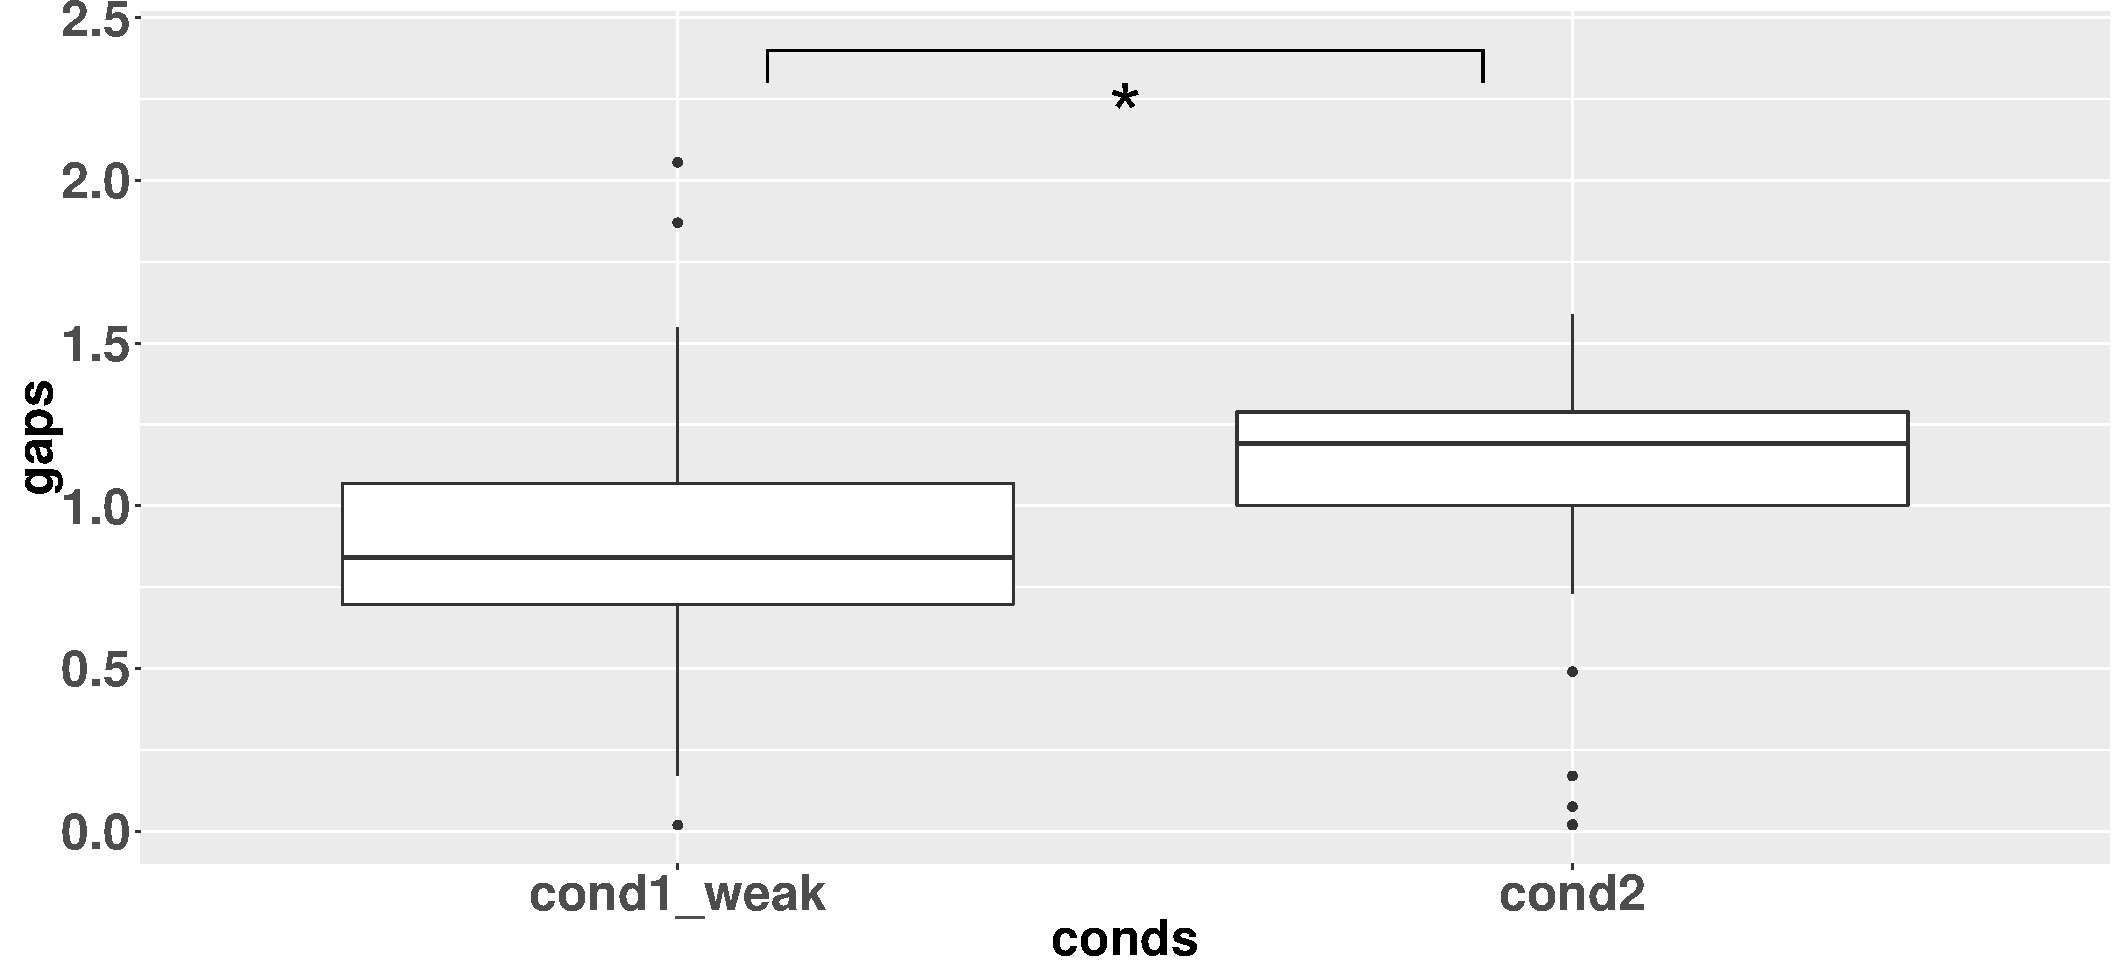
\includegraphics[width=\linewidth]{figure/boxTransitionsUA.pdf}
\caption{Durations of silence during User to Agent transitions (gaps in seconds).}
\label{box_ua}
\end{figure}

\begin{figure}
\centering
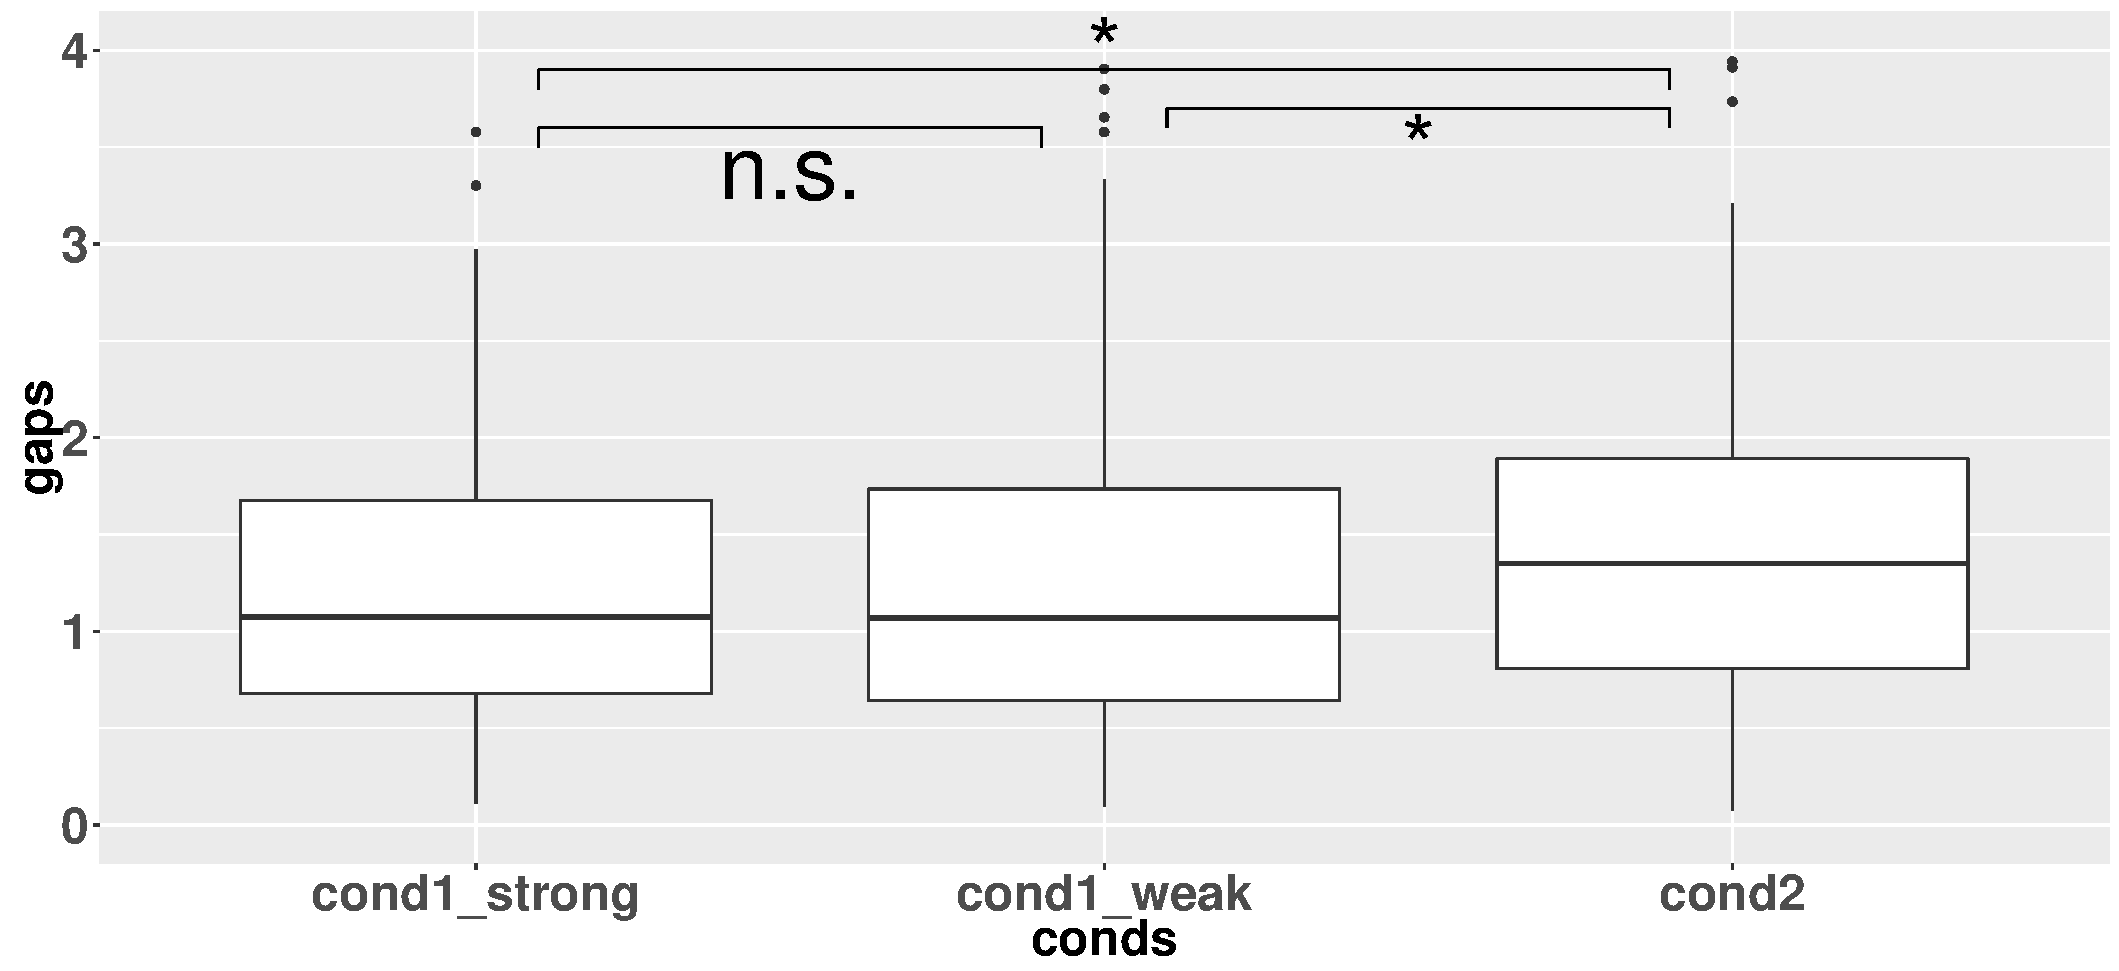
\includegraphics[width=\linewidth]{figure/boxTransitionsAU.pdf}
\caption{Durations of silence during Agent to User transitions (gaps in seconds).}
\label{box_au}
\end{figure}


We completed the analysis of the subjective evaluations with an objective analysis of the interaction. 
We first analyzed the duration of the transitions, distinguishing user to agent transitions from agent to user ones (Figures \ref{box_ua} and \ref{box_au}).
For this analysis, we annotated manually the turns of the different participants and aligned the loudness profile of the participants to the annotations we made. We kept only transitions that were not overlaps and transitions that were not anticipated by the agent. We observed first a high number of mistakes in the detection of user's end of turns, whatever the condition, with almost 50 \% of transitions having at least slight overlaps.  
%The repartition of the user to agent transitions is shown on figure \ref{box_ua}, and the repartition of agent to user transitions is shown on the figure \ref{box_au}. 

These results show that for the condition 1 the agent took the turn more rapidly (average: 840 ms) compared to the second condition (1.19 s), the difference being significant (p$<$0.05). The difference was also significant (p$<$0.05) for the agent-user transitions: in condition 1 the mean duration of silence was 1.11 s and 1.39 s for the second one. 
In addition, the pitch of the user was significantly greater than her mean pitch during conflictual moments, for condition 1 Strong. This mean that the user seemmed to react in a specific manner to the interruptions made on purpose by the agent in ``condition 1 strong". Such reaction could not be observed in the other conditions where the agent overlapped involuntarily the user's speech.
 %to these transition duration values, the pitch variation of the participants was measured during interruptions by the agent. The results showed that the pitch of the user was significantly greater than the mean pitch of the participant during conflictual moments, for the condition 1 ``Strong".

% Comment peut-on expliquer que la durée moyenne de transition soit le double du seuil de détection de la fin de tour de l'utilisateur ?
% À faire : valeur moyenne de pitch supérieure aussi lors des overlaps de l'agent pour les autres conditions, différences de perception qui pourrait laisser penser une différence de traitement ?
% Comportement de l'agent : est-ce que l'utilisateur a beaucoup interrompu l'agent ?


\subsection{Discussion}

Results show that our model improve the ability of the agent to coordinate turns with users. Indeed, while unvolontary overlaps due to mistakes in the perception of the user end of turn do not seem to differ between conditions, the agent took the turn faster in ``condition 1 weak" compared to ``condition 2". The high rate of end of turn false detections by the two models (50 \% of user-agent transitions) can be partially explained by the voice activity detector used to detect the moments were the user spoke, showing an important number of moments were no voice was detected whereas the user actually spoke. 
However, responses to questions Q1, Q2, Q6 and Q7 show that users didn't perceive this improved ability to coordinate turns. The fact that the participants seemed not disturbed by the relatively high silence duration of user to agent transitions support the idea that the latter did not expect optimal turn transitions from the agent.

Moreover, when investigating if the signals displayed by the agent were correctly perceived by the user, we observed that users considered almost equally that the agent both interrupted them unvolontarily and interrupted them on purpose both in ``condition 1" when the agent raises volume and pitch to inform the user about its intention to grab the turn and in ``condition 2" when no variation of pitch and volume are made. However, when analyzing the user's behavior, we found that the latter increased pitch when interrupted by the agent only in ``condition 1 strong". This lead us to think that users distinguish at least implicitly the volontary or unvolontary character of the interruptions and varied its reaction accordingly. This conducts us to think that solely raising pitch and loudness did not seem to sufficiently inform the agent's intention to grab the turn. The lack of distinction between interruptions, those that were due to mistakes in the detection of the user end of turn and those that were voluntary could be due to difficulties of the participants to perceive the prosodic variations of the agent. These difficulties could come from the quality of the tts voice we used, participants having often reported the bad quality of the voice. 
At the end of the experiment, we collected the oral impressions of the participants on the interaction. We also observed that participants were divided when asked about their perception of the agent's interruptions. Six participants explicitly mentionned that they perceived the interruptions of the agent as non-voluntary, on the opposite, thirteen participants perceived at least some interruptions as voluntary. 

We also analyzed the way the agent signals at the end of turn helped users coordinate with the agent. As a result, we found that users took the turn faster after the end of the agent's turn in ``condition 1" compared to ``condition 2". Two hypotheses can be made to explain this variation in behavior. First, the user could have perceived the decrease in pitch and loudness made by the agent to inform its intention to release the turn, this perception helping the user to identify the agent's end of turn. Second, variations in agent-user transition durations could be the result of an alignment effect: the fact that the agent took the turn faster made the user take the turn faster. This hypothesis is plausible, as such alignment has been observed in human conversations \citep{levitan_entrainment_2015}.  

Finally, the results of our questionnaire do not permit to conclude about the effect of varying turn-taking behaviors to the user's judgements about the agent's credibility, user's satisfaction and easiness to interact with the agent, as answers to questions Q8, Q9, Q10 and Q11 are not significantly higher for condition 1 compared to condition 2. Moreover, answers to these questions do not strongly favorize positive impressions about the agent. However, oral impressions collected after the interaction are not so categorical.   
For example, perception of the interruption seems to conduct to more positive impressions about the interaction for some participants. Four participants judged interruptions as coherent and credible given the dialog context, and five participants associated these interruptions to the fact that the agent did not agree or tried to impose its own ideas. Finally, among those thirteen participants, five participants judged those interruptions as humanlike. On the oppoposite, one of the participants we interviewed after the experiment reported a rage feeling linked to the incessant interruptions of the agent, and two participants reported that they were annoyed by these interruptions. We could explain differences in the impressions given by interruptions by the fact that the agent interrupted the user regardless of the dialog context. This could results in moments where the agent's interruptions seemed not credible given the dialog context while other interruptions were particularly relevant given the dialog context. Interruptions could thus give an impression of smoothness and immersion in the dialogue to the condition that they should be made coherently with the dialog context. 



